\section{Actual staged construction in the original scientist world}
\label{sec:native-staged-construction}
\subsection{Free design, component observations and whole-world evaluation}
We next execute the staged interface with the local 35B designer and original
Qwen3-8B scientists, rather than attributing the preceding scripted software
behavior to an autonomous author. Source \code{f47270b9} preserves the original
corpus, persistent four-year world, fixed T/U losses, R7-only initial optimizer
reference and comparison-only hand timing control. Three proposals per
objective are interleaved T0,U0,U1,T1,T2,U2. Arbitrary mechanism source, nodes,
ports, protocols, connections and schedules remain expressible in the general
native interface. There is no novelty, fairness or improvement admission test.

The designer can inspect and edit its literal draft, observe no-network
component execution on 20 historically recorded R7 inputs, revise and explicitly
finish. Eligible edited code is tested against its four original yearly inputs;
new interfaces remain legal but may be untested. Failed component returns do
not veto submission. All component tests and HTTP calls share a finite worker
allowance; the host neither repairs source nor supplies a missing consumer.
Each proposal permits at most 16 model steps and 64 probes. Initial and per-
proposal directed readiness tests remain separate from free-design evidence.

\begin{table}[htbp]
\centering\small
\begin{tabular}{lrrrl}
\toprule
System/slot & T & U & Probes & Actual own edit\\
\midrule
R7 original & $-18$ & $-13.3333$ & --- & Reference\\
Hand timing & $-20$ & $-15.3333$ & --- & Reference\\
T0 & $-18$ & $-13.3333$ & 8 & Selection source\\
U0 & $-18$ & $-13.3333$ & 0 & Literal retention\\
U1 & $-18$ & $-12$ & 16 & Agenda source\\
T1 & $-18$ & $-13.3333$ & 4 & Selection source\\
T2 & $-18$ & $-13.3333$ & 20 & Selection source\\
U2 & $-18$ & $-13.3333$ & 16 & Selection source\\
\bottomrule
\end{tabular}
\caption{All eight completed physical worlds in the actual staged study.
Both losses are minimized; the hand is comparison-only. All 64 component
attempts return, without an error-repair demonstration. No own graph adds
nodes or connections. Display rounding does not enter selection. Five own
outcomes tie R7 and U1 worsens content utility; none beats the hand.}
\label{tab:actual-staged-development}
\end{table}

\begin{figure}[htbp]
\centering
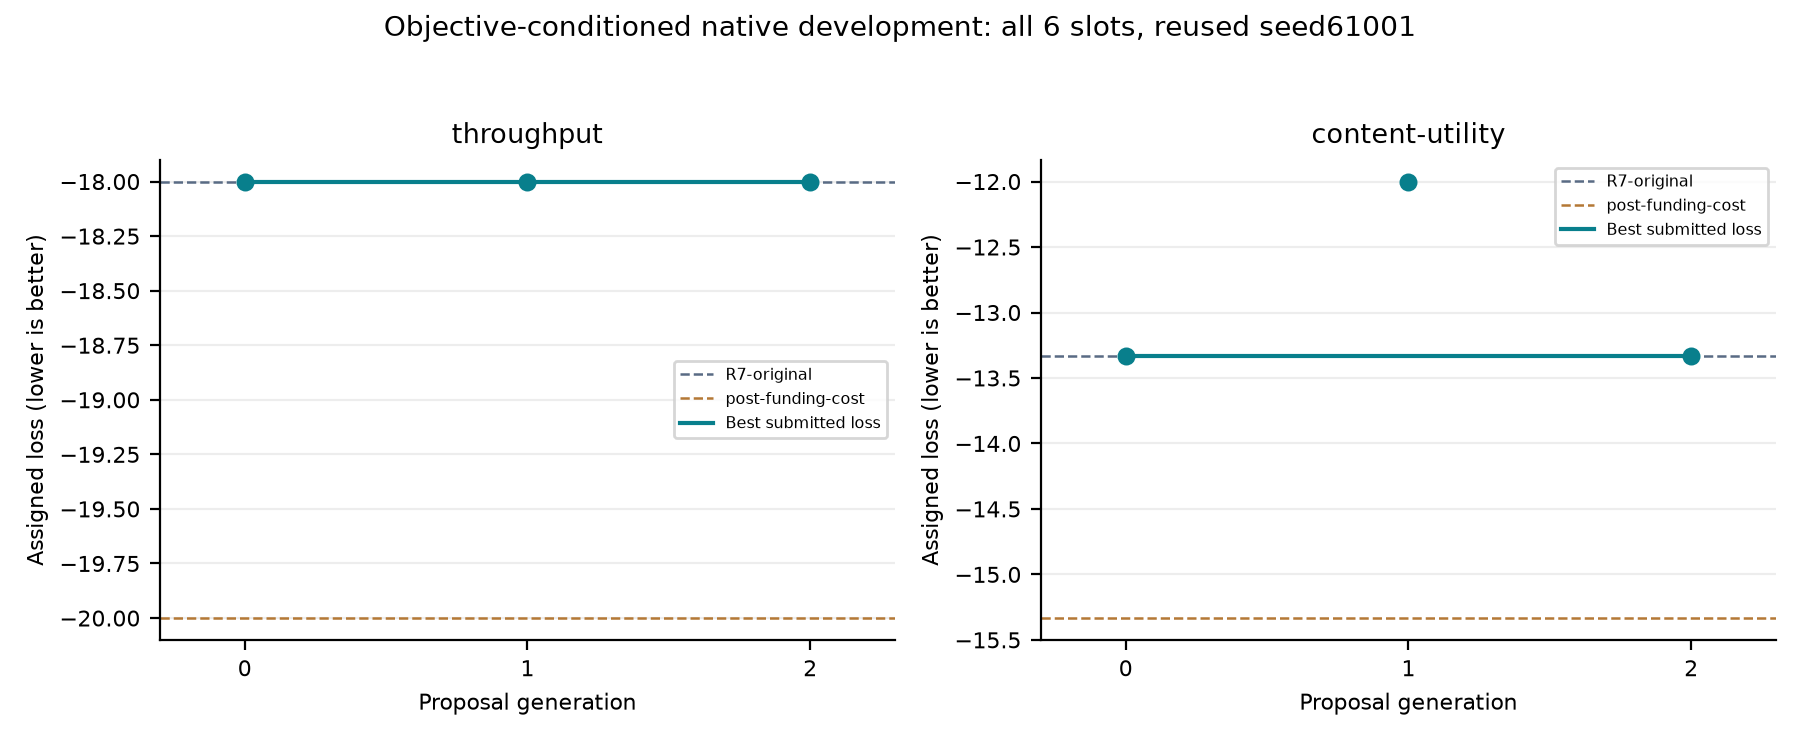
\includegraphics[width=\linewidth]{figures/native-staged-construction-v1/objective-loss-paths.png}
\caption{The actual objective-conditioned staged development paths on reused
seed 61001. Markers are all three completed own proposals per objective;
solid lines retain best submitted loss, and dashed lines show both controls.
The U1 marker is worse while the best-own line stays flat. Neither objective
improves over its optimizer-visible R7 reference, and the comparison-only hand
remains better. This is one development history without independent error bars.}
\label{fig:actual-staged-development-paths}
\end{figure}

\subsection{Execution is not improvement or an invented graph}
All six proposals and eight native worlds complete. Each proposal consumes 14
actual model steps, for 84 total, including rejected actions and explicit finish.
The 64 probe returns do not constitute 64 independent scientific evaluations.
T0/T2/U2 change selection source, T1's selection AST equals R7, and U0
explicitly retains the literal parent. No new mechanism or connection is
generated. This is a completed construction-and-evaluation path, not an
automatic discovery of the hand timing rule or an isolated feedback benefit.

U1 changes agenda code to prefer smaller declared project duration with a
keyword-count tie heuristic. The 23rd scientist request changes its research
topic from distributed systems to software engineering. The two worlds accept
18 occurrences each: 12 shared, full-rating-identical occurrences contribute
utility 8; the six R7-only occurrences contribute $16/3$, while the six U1-only
occurrences contribute 4. Thus its U loss worsens by $4/3$ despite equal T.
This diagnoses observed content replacement, not a causal advantage of a
proxy for topic quality. The heuristic is authored code, not a changed loss.

The actual U1 planning frame contains the exact U arithmetic but lacks its
inline semantic definition; the inspected T2 frame includes a count definition.
The full measurement contract remains retrievable in the request archive,
and U1's recorded reads do not request that archive. This is a bounded
information-presentation limitation, not proof that a target was absent, an
API was broken or that the omission caused the unfavorable result. The study
does not isolate an equal-information objective intervention. Prospective
interface corrections do not retrospectively repair its inputs or failures.

\subsection{Complete costs, frozen selection and remaining evidence}
Two original-source audits and cost projections agree byte for byte; all
files in the paired result, choice, effect, request-class and construction
exports also agree. These are reconstructions of one development history,
not independent optimizer replications. Scientist caches contain 937 complete
responses, 1,117,688 prompt and 98,457 completion tokens, with no input lacking
a committed reply. The 190,032 cached prompt tokens are a subset. Separately
recorded calls include 200 readiness, 84 proposal steps, 13 designer loads,
eight scientist loads and 93 physical content-critic requests. Missing load
usage stays unknown. Campaign wall time is 13,394.180 seconds on the shared
host, including construction and readiness, not dedicated inference speed.

The unchanged own-only minimum/chronological-first-tie rule selects T0 for T
and U0 for U. U0 is literally R7, not a fallback. Before own outcomes, a
prospective note declares unused seed 1891355522; it is retained regardless
of the absence of development improvement. Broad production-journal inventories
and an immediate pre-dispatch repeat find no prior use, with only exact
hash-bound nonproduction fixtures excluded. Four logical labels require three
literal-distinct physical jobs, with no new author, repair or reselection.
That fixed evaluation has started but is not complete at this source snapshot;
no held-out score or independent replication is asserted here.

Completing all construction slots removes an important technical missingness
in this study, but does not supply an important general objective-to-institution
answer. The negative own result, absent topology exploration and unequal inline
information coverage remain explicit. Simply repeating this question at larger
scale would not by itself establish main-track significance.
\FloatBarrier
